\documentclass[amssymb,twocolumn,prd,nofootinbib,showpacs]{revtex4-1}

\usepackage{graphicx}  % needed for figures
\usepackage{dcolumn}   % needed for some tables}
%\usepackage[style=authoryear,backend=biber]{biblatex}
\usepackage{bm}        % for math
\usepackage{amsmath,amssymb}
%\usepackage{natbib}
\usepackage{hyperref}
\usepackage{color}
\definecolor{purple}{rgb}{0.58,0.0,0.83}
\usepackage{caption}
\usepackage[toc,page]{appendix}
\usepackage{bm}        % for math
\usepackage{amsmath,amssymb}
\usepackage{hyperref}
\usepackage{color}
\definecolor{purple}{rgb}{0.58,0.0,0.83}
\usepackage{caption}
\usepackage[toc,page]{appendix}
\usepackage{subcaption}
\newcommand{\jav}[1]{\textcolor{red}{(jav: #1)}}


\begin{document}

\title{On the two field inflationary models and constraints for ultra-light scalar field dark matter spectators during inflation}
\author{Luis E. Padilla}  
\email{epadilla@fis.cinvestav.mx}
\affiliation{Departamento de F\'isica, Centro de Investigaci\'on y de Estudios Avanzados del IPN, 
A.P. 14-740, 07000 M\'exico D.F.,  M\'exico.}
   \author{J. Alberto V\'azquez}  
\email{javazquez@icf.unam.mx}
\affiliation{Instituto de ciencias f\'isicas, Universidad Nacional Aut\'onoma de M\'exico, sede Cuernavaca, 
Morelos, M\'exico}
\author{Tonatiuh Matos}  
\affiliation{Departamento de F\'isica, Centro de Investigaci\'on y de Estudios Avanzados del IPN, A.P. 14-740, 
07000 M\'exico D.F.,  M\'exico.}
   \author{Gabriel Germ\'an}  
\affiliation{Instituto de ciencias f\'isicas, Universidad Nacional Aut\'onoma de M\'exico, sede Cuernavaca, 
Morelos, M\'exico}

\date{\today}

\begin{abstract}
Cosmological inflation is nowadays the most accepted mechanism to explain the  primordial seeds 
that led to  the structure formation observed in the Universe. Current observations are in well agreement 
to initial adiabatic conditions, which implies that  single-scalar-field inflation may be enough to describe 
the early Universe. 
%
However, there are several scenarios where more than a single field could be relevant during inflation. 
The simplest situation is where the so-called spectator is present. 
In this paper we initially review the formalism for two field inflationary models and then to apply it to two different 
spectator scenarios. Firstly, to the possibility that an ultra-light scalar field dark matter coexist with the inflaton, 
where such ultra-light field could be auto-interacting or only massive. Secondly, to the curvaton scenario.
In both cases we provide a comparison to current cosmological data.    
\\
\jav{cuesta un poco de trabajo identificar que ya se obtuvo en otros articulos y que se obtiene aqui. 
Tratar de poner enfasis en lo nuevo.}
\jav{Hay muchos 'consider', 'scalar field', 'start', 'scenario', 'notice', 'in this way', 'we can', 'using', 
agregar sinonimos o cambiar frases.}
\jav{Acomodar secciones, subsecciones, subsubsubsecciones}
\jav{obtienes constricciones en terminos de $r$, y no vuelves a mencionar $n_T$. mencionar algo sobre este numero.}
\end{abstract}
\pacs{????}
\begin{keywords}
a Inflation  --  Isocurvature  --  Scalar field -- Dark Matter
\end{keywords}

\maketitle


%%%=========================================================================%%%
\section{Introduction}
\label{introduction}
%%%=========================================================================%%%

It is well accepted that primordial seeds, of the structure formation in the Universe, were generated by quantum 
fluctuations provided by a scalar field (SF) during an inflationary era. 
The simplest scenario where density perturbations are carried out by a single inflaton is quite preferred 
since the initial perturbations are nearly adiabatic \cite{const1,const2,planck}. However, the presence of any 
light field, other than the inflaton, could also fluctuate during inflation and contribute to the primordial density 
perturbations. 
%
Also, by assuming extra scalar sources during inflation may help to relax restrictions in inflationary models
\jav{por que they are preferred in a model construction point of view?}.
%The fact that we should consider extra scalar sources during inflation is because they are prefered 
%in a model construction point of view and they can help to relax restrictions in inflationary models. 
For instance, we could consider scenarios where extra degrees of freedom are generated by ``spectator" 
fields that are not dynamically important during inflation or scenarios where more than one SF drives inflation 
during the early Universe. 
%
Whichever scenario we assume it has to fulfill the simplest constraints of any inflationary model, given in 
terms of the spectral index $n_R$, the tensor-to-scalar ratio $r$ and the current limits imposed on the 
isocurvature perturbations. 
\\

We assume two spectator field scenarios.
%
%In the spectator field scenario we can consider at least two models that are important to study. 
Firstly, we consider the possibility that an extra SF may coexist with the inflaton and be used as a dark 
matter component (DM). 
%
The idea of scalar fields as DM was initially introduced by \cite{SF1} and since then rediscovered 
using different names, for instance Scalar Field Dark Matter  (SFDM)  \cite{SF2},  Fuzzy  DM  \cite{SF3}, 
Wave DM \cite{SF4,SF5}, Bose-Einstein Condensate DM \cite{SF6} or Ultra-light Axion DM \cite{SF7,SF8}, 
amongst many others. 
%
The purpose of this field is to resolve the apparent conflict, with observations, that exhibits the
cold dark matter (CDM) formed of weakly-interacting massive particles (WIMPS) \cite{LCDM1,LCDM2}. 
%was proposed due to the fact that the preferable model, which considers the DM as cold and assumes to be formed 
%of weakly-interacting massive particles (WIMPS) \cite{LCDM1,LCDM2}, is in apparent conflict with observations on 
Some of these weaknesses may appear at small-scales within galaxies, e.g. cuspy halo density profiles, overproduction of 
satellite dwarfs within the Local Group and many others, see for example \cite{problem1,problem2,problem3,problem4,problem5}). 
Since then, the SFDM model has been successfully tested by different observations;  
for a review on ultra-light SFDM see \cite{SF9,SF10,SF11,SF12}. 

Secondly, we analyze the possibility that the spectator field, a curvaton, contributes to the primordial adiabatic curvature 
perturbations \cite{curv1,curv2,curv3} \jav{the curvaton is a SF? or what's the difference with the previous case. 
%
The SFDM could also contribute to the adiabatic curvature perturbations?  Escribir que diferencias tienen ambos casos}. 
This scenario is of a particular interest because in the limit where all primordial adiabatic 
perturbations are generated by the curvaton, the inflaton is completely free and just constrained 
\jav{quien es constrained?, si es el
inflaton entonces que importancia tiene este caso. Si es el curvaton explicar.} by the inflationary mechanism.
\jav{Por que el curvaton no puede ser SFDM? o al reves.}

This paper is organized as follows: First, in section \ref{Generalities} we review the formalism of two-field 
inflationary models. 
Then in section \ref{experimentos} we present the basic inflationary observables used to constraint our models. 
Once the mathematical background and the observational restrictions are given, in section \ref{simplest} we 
analize two different models. 
First, we assume the presence of a scalar field dark matter (SFDM) spectator during inflation, where the  
 field could be either massive or auto-interacted. We provide some limits for the SFDM free parameters and 
 compare them with the actual constraints given by astrophysical and cosmological observations. 
 Then we review the typical curvaton quadratic model with a chaotic-like inflationary potential. We show how these 
 kind of models help us to relax the inflationary potentials and we constraint it with last data given by 
 Planck 2018 \cite{planck}. Finally in section \ref{conclusions} our conclusions are given.      

%%%=========================================================================%%%
\section{Generalities for two field inflationary models}\label{Generalities}
%%%=========================================================================%%%


In this section we review the two-field inflationary models for inflation, following \cite{twofields}. 
\jav{toda la seccion se extrajo de ese art? son casi dos paginas!.}
%
\subsection{Background equation of motion}

We consider a two-field inflationary model with canonical kinetic term and  its dynamics being described by an arbitrary 
interacting potential $V(\phi,\psi)$. The classical fields are real, homogeneous and evolve in a FLRW background. 
Then, the background equations of motion for each scalar field and the Hubble parameter are given by
%
\begin{subequations}
\begin{equation}\label{KGEq}
\ddot{\phi}_i+3H\dot{\phi_i}+\frac{dV_i}{d(\phi_i)^2}\phi_i=0 \ \ \ (i=\phi,\psi),
\end{equation}
\begin{equation}
H^2=\frac{8\pi G}{3}\left[V+\frac{1}{2}\left(\dot{\phi}+\dot\psi\right)\right].
\end{equation}
\end{subequations}

During the inflationary era it is assumed that each of the scalar fields satisfy the slow-roll conditions, and 
this happens always that $\epsilon_i,|\eta_{ij}|\ll 1$; $\epsilon_i$ and $\eta_{ij}$ are called the slow-roll parameters 
and are defined in appendix [A]. If this happens we can rewrite the above equations as
%
\begin{subequations}
\begin{equation}\label{eq:in_1}
\dot{\phi}_i\simeq \frac{2}{3}\epsilon_i V,
\end{equation}
\begin{equation}\label{eq:in_2}
H^2\simeq \frac{8\pi G}{3}V\left(1+\frac{1}{3}\epsilon^H\right),
\end{equation}
\end{subequations}
%
where $\epsilon^H$ is a new slow-roll parameter defined in appendix [A]. 
The set of differential equations, (\ref{eq:in_1}) and (\ref{eq:in_2}),  
describes the classical dynamics of bout scalar fields during the inflationary era.

%%%-------------------------------------------------------------------------------------------%%%
\subsection{Adiabatic and Isocurvature perturbations}
%%%-------------------------------------------------------------------------------------------%%%


The equation of motion for the perturbed fields, in the spatially flat gauge, are
%
\begin{equation}
\ddot{\delta\phi}_i+3H\dot{\delta\phi}_i+\sum_j\left[V_{ij}-\frac{8\pi G}{a^3}\frac{d}{dt}\left(\frac{a^3}{H}\dot{\phi}_i \dot\phi_j\right)\right]\delta\phi_j=0.
\end{equation}
%
For large scales ($k\ll aH$) \jav{and for small scales? or what'd be the difference?} it is better to work in a 
rotating basis of the fields given by
%
  \begin{subequations}
  \begin{equation}
  \binom{\delta \sigma}{\delta s}=S^{\dagger}\binom{\delta \phi}{\delta\psi},
  \end{equation}
  with
  \begin{equation}\label{angle}
  S=\begin{pmatrix}\cos\theta & -\sin\theta\\ \sin\theta & \cos\theta\end{pmatrix}, \ \ \ \tan\theta =\frac{\dot \psi}{\dot \phi}\simeq\pm \sqrt{\frac{\epsilon_\psi}{\epsilon_\phi}}.
  \end{equation} 
  \end{subequations}
  %
The field $\sigma$ is parallel to the trajectory of the field space and  
usually called \textit{adiabatic field}, while the field  $s$ is perpendicular and called \textit{entropy field}. 
%
If the background trajectory is curved then $\delta\sigma$ and $\delta s$ are correlated at the Hubble exit. 
In this way the power spectrum and cross-correlation at Hubble exit is given by
\begin{subequations}
\begin{equation}
P_{\sigma^*}(k)\simeq\left(\frac{H_*}{2\pi}\right)^2(1+(-2+6C)\epsilon-2C\eta_{\sigma\sigma}),
\end{equation}
\begin{equation}
C_{\sigma s^*}(k)\simeq-2C\eta_{\sigma s}\left(\frac{H_*}{2\pi}\right)^2,
\end{equation}
\begin{equation}\label{5c}
P_{s^*}(k)\simeq\left(\frac{H_*}{2\pi}\right)^2(1+(-2+2C)\epsilon-2C\eta_{ss}),
\end{equation}
\end{subequations}
%
where $C\simeq 0.7296$ and $\epsilon$ and $\eta_{ij}$ ($i,j=\sigma,s$) are new slow-roll parameters 
defined in term of the new adiabatic and entropy fields (see appendix [A]). Here quantities measured at 
hubble exit are labeled by $^*$.

%%%-------------------------------------------------------------------------------------------%%%
\subsection{Power spectrum and spectral indices}
%%%-------------------------------------------------------------------------------------------%%%

The curvature and isocurvature perturbations are defined as
%
\begin{equation}\label{RS}
R\equiv\frac{H}{\dot\sigma}\delta \sigma, \ \ \ S=\frac{H}{\dot \sigma}\delta s.
\end{equation}
%
In the slow-roll limit and large scales \jav{again large scales}, the evolution of curvature and isocurvature 
perturbations can be written using the formalism of transfer matrix as
%
\begin{equation}
\binom{R }{S}=\begin{pmatrix}1 & T_{RS}\\ 0& T_{SS}\end{pmatrix}\binom{R}{S}_*,
\end{equation}
where
\begin{subequations}
\begin{equation}
T_{SS}(t^*,t)=\exp\left(\int^t_{t^*}\beta Hdt'\right), \ \ \
\end{equation}
\begin{equation}\label{TRS}
T_{RS}(t^*,t)=\exp\left(\int^t_{t^*}\alpha T_{SS}Hdt'\right),
\end{equation}
\end{subequations}
%
and at linear order in slow-roll parameters
%
\begin{equation}
\alpha\simeq -2\eta_{\sigma s}, \ \ \ \ \beta\simeq-2\epsilon+\eta_{\sigma\sigma}-\eta_{ss}.
\end{equation}

The primordial curvature perturbation right after inflation has ended is given in large scales \jav{again large scales} by
%
\begin{equation}
R=\Psi+\frac{H\delta\rho}{\rho},
\end{equation}
%
where $\Psi$ is the gravitational potential. The conventional definition of the isocurvature 
perturbation for an $i$ specie is given relative to the radiation density by
%
\begin{equation}
S_i=H\left(\frac{\delta\rho_{i}}{\rho_{i}}-\frac{\delta\rho_\gamma}{\rho_\gamma}\right).
\end{equation}
%
Then, the final power spectra, at the beginning of the radiation-domination era, are thus
%
\begin{subequations}\label{spectrums}
\begin{equation}\label{PRf}
P_R\simeq P|_*(1+\cot^2\Delta),
\end{equation}
\begin{equation}\label{isosecond}
P_S=T^2_{SS}P|_*,
\end{equation}
\begin{equation}
C_{RS}=T_{RS}T_{SS}P_R|_*,
\end{equation}
\end{subequations}
%
where at linear order in slow-roll parameters
%
\begin{equation}
P|_*=\frac{1}{2\epsilon}\left(\frac{H_*}{2\pi M_{pl}}\right)^2,
\end{equation}
%
with $M_{pl}=1.221\times 10^{19}GeV$ the Planck mass and $\Delta$ is the observable correlation angle 
defined at lower order as
%
\begin{equation}
\cos\Delta =\frac{T_{RS}}{\sqrt{1+T_{RS}^2}}.
\end{equation}
%
The final spectral indices, defined as $n_x-1=d\ln P_x/d\ln k$, at linear order in slow-roll parameters are
%
\begin{subequations}\label{tilts}
\begin{eqnarray}
n_R-1&\simeq & -(6-4\cos^2\Delta)\epsilon+2\sin^2\Delta\eta_{\sigma\sigma}\nonumber \\ &&+4\sin\Delta\cos\Delta\eta_{\sigma s}+2\cos^2\Delta\eta_{ss}\\
n_c-1&\simeq &-2\epsilon+2\tan\Delta\eta_{\sigma s}+2\eta_{ss}\\
n_S-1&\simeq & -2\epsilon+2\eta_{ss}.
\end{eqnarray}
\end{subequations}

In order to understand the contribution of each field to the primordial spectrum, we rewrite the primordial adiabatic 
and entropy perturbations on super-horizon scales \jav{is this valid at all scales?} as a power law, given by
%
\begin{subequations}\label{PswAs}
\begin{equation}\label{PrAs}
P_R=A_r^2\left(\frac{k}{k_0}\right)^{n_{ad1}-1}+A_s^2\left(\frac{k}{k_0}\right)^{n_{ad2}-1},
\end{equation}
\begin{equation}\label{PrCrs}
C_{RS}=A_sB\left(\frac{k}{k_0}\right)^{n_{cor}-1},
\end{equation}
\begin{equation}\label{PsAs}
P_s=B^2\left(\frac{k}{k_0}\right)^{n_{iso}-1},
\end{equation}
\end{subequations}
%
where at linear order $n_{ad1}=-6\epsilon+2\eta_{\sigma\sigma}$, $n_{ad2}=2n_C-n_S$, 
$n_{cor}=n_c$, $n_{iso}=n_S$. We have that $A_r^2$, $A_s^2$ and $B$ can be written in 
terms of the correlation angle $\Delta$ as

\begin{subequations}
\label{RelAs}
\begin{equation}
A_r^2=[P_R\sin^2\Delta]_{k_0}, \ \ \ \ A_s^2=[P_R\cos^2\Delta]_{k_0},
\end{equation}
\begin{equation}
B^2=[T_{SS}^2 P_R|_*]_{k_0}.
\end{equation}
\end{subequations}
%
$A_r^2$ and $A_s^2$ are the contributions of the adiabatic and entropy fields to the amplitud 
of the primordial adiabatic spectrum. 

%%%-------------------------------------------------------------------------------------------%%%
\subsection{Gravitational waves}
%%%-------------------------------------------------------------------------------------------%%%

Given the fact that scalar and tensor perturbations are decoupled at linear order, the amplitude of 
the gravitational waves spectrum at horizon crossing 
%is the same than the single-field case and the gravitational waves amplitude 
remained frozen on large scales after the Hubble exit during inflation. 
In this way the power spectrum and the tilt of the gravitational waves are given by
%
\begin{equation}
P_T=P_{T*}\simeq 8 \left(\frac{H_*}{2\pi M_{pl}}\right)^2(1+2(-1+C)\epsilon),
\end{equation}
\begin{equation}\label{tiltsnt}
n_T\simeq -2\epsilon\left[1+\left(\frac{4}{3}+4C\right)\epsilon+\left(\frac{2}{3}+2C\right)\eta_{\sigma\sigma}\right].
\end{equation}

Then the tensor-to-scalar ratio ($r$) at Hubble exit is the same than in a single field scenario. 
However, at super-horizon scales, the curvature perturbations continue evolving as \eqref{PRf}. 
Therefore the tensor-to-scalar ratio some time after the end of inflation is
%
\begin{equation}\label{Tensortoscalar}
r\simeq 16\epsilon \sin^2\Delta\left[1-\left(\frac{4}{3}+4C\right)\epsilon +\left(\frac{2}{3}+2C\right)\eta_{\sigma\sigma}\right].
\end{equation}
Notice that the single SF case works as an upper constraint on $r$, that can be tested by observations.

%%%=========================================================================%%%
\section{Constraints on inflationary parameters}\label{experimentos}
%%%=========================================================================%%%

In the standard approximation the inflationary observables are given by the tensor to scalar ratio $r$, 
the spectral index for adiabatic perturbations $n_R$ and the amplitude for adiabatic perturbations $A_r^2$.  
The constraints of these parameters are quoted at the pivot scale $k_0=0.05 Mpc^{-1}$ 
by \cite{const1,const2,planck,const3,const4,const5}
%
\begin{subequations}
\begin{equation}\label{amplitude}
A_r^2(k_0)=(2.215^{+0.032}_{-0.079})\times 10^{-9}, \ \ \ \text{at $68\%$ CL},
\end{equation}
\begin{equation}
r_{k_0}<0.08 \ \ \ \text{at $95\%$ CL},
\end{equation}
\begin{equation}\label{n_R}
n_R(k_0)=0.968 \pm 0.006.
\end{equation}
\end{subequations}
%
Using these measurements we are able to constrain the value of the Hubble expansion rate during 
inflation $H_*$ as \cite{H1,H2}
%
\begin{equation}\label{Hinf}
r = 1.6\times 10^{-5}\left(\frac{H_{inf}}{10^{12}GeV}\right)^2.
\end{equation}

As we have seen beforehand, if more than one SF is present during inflation we will obtain isocurvature 
perturbations generated by extra scalar fields perpendicular to the trajectory on field space. 
%
Parameterizing the isocurvature power spectrum for dark matter in terms of the curvature power as
%
\begin{equation}\label{isoCDM}
P_{DM}(k) = \frac{\beta_{iso}(k)}{1-\beta_{iso}(k)}P_R(k),
\end{equation}
%
where $P_{DM}=\delta \rho_{DM*}/\rho_{DM}$, $\delta\rho_{DM}$ are the isocurvature 
perturbations for the dark matter ($DM$) generated by extra scalar fields during inflation and $\rho_{DM}$ 
is the initial condition of DM. 
The uncorrelated scale-invariant DM isocurvature is constrained by Planck data \cite{const1,const2} 
at pivot scale $k_0$ as
%
\begin{equation}\label{betaiso}
\beta_{iso}(k_0)<0.038 \ \ \ \text{at $95\%$ CL}.
\end{equation}
%
Notice that isocurvature perturbations can be used to constraint the inflationary scale, 
just by combining equations \eqref{Hinf}, \eqref{isoCDM} and \eqref{betaiso}.
%
%
%
%%%=========================================================================%%%
\section{Simplest scenario: The single-field scenario and constraints for SFDM models}\label{simplest}
 \jav{pq single-field? esSFDM/curvaton + inflation?}
%%%=========================================================================%%%

The simplest scenario to assume is that only one scalar field was dynamically important during inflation and 
the extra field observer contributed to the primordial spectrum by generating only isocurvature fluctuations. 
%
This scenario is obtained always that $\rho_{\psi}\ll \rho_{\phi}$ during all of the inflationary period, 
where $\phi$ describes the inflaton. 
%
Even tough the idea of adding an spectator, that does not contribute to the inflationary process 
\jav{does not contribute in any possible way?}, could be considered as unnecessary, there are at least 
two scenarios where  extra degrees of freedom can be important. 
%
One is by considering an scenario where this extra scalar field can be used as a DM candidate, 
in such case we will have isocurvature constraints for our model. On the other hand we have the so 
called curvaton inflationary model, where this new field is responsible for the majority of the adiabatic 
perturbations produced during inflation. This scenario has been well studied in the literature \jav{si ya ha sido 
bien estudiado, por que considerarlo aqui? que hay nuevo?} being 
one of the preferable scenarios for the inflationary process \cite{curvaton15,curvaton16}. 

%%%-------------------------------------------------------------------------------------------%%%
\subsection{SFDM spectator scenario}
%%%-------------------------------------------------------------------------------------------%%%

In this scenario we require that the SFDM candidate be a stable spectator field with negligible 
classical dynamics and energy density during inflation. 
We can obtain such scenario by considering that the trajectory in the field space evolves in the inflaton 
direction $\phi$ whereas the direction perpendicular to the trajectory corresponds to the SFDM $\psi$. 
Notice that it is necessary \jav{pq necesario? o de donde se ve?} that our dark matter candidate evolves 
much slower than the inflaton and its density be smaller than the associated to the inflaton. 
Then, we can see that the last conditions demand that $\epsilon_\psi\ll \epsilon_\phi$.

During the inflationary scenario the entropy and adiabatic perturbations are uncorrelated which 
implies that $T_{RS}=0$ (and $C_{RS}=0$) as can be seen from \eqref{TRS} imposing initial conditions 
at horizon crossing. In this way we have that $\cos\Delta =0$. 
Also, as expected from \eqref{PrAs} and \eqref{RelAs}, the primordial power spectrum for the adiabatic 
perturbations is produced purely by the inflaton (i.e. $A_s=0$) while quantum fluctuations of the SFDM 
give rise to the generation of uncorrelated isocurvature perturbations. 
%In this way the primordial power spectrum of adiabatic, isocurvature and tensor perturbations are
%\begin{subequations}
%\begin{equation}
%P_R=P_R|_*
%\end{equation}
%\begin{equation}\label{PS1}
%P_s=T_{SS}^2 P_R|_*
%\end{equation}
%\begin{equation}
%P_T=\frac{8}{M_{pl}^2}\left(\frac{H_*}{2\pi}\right)^2
%\end{equation}
%\end{subequations}
%and from \eqref{tilts} and \eqref{tiltsnt} the tilts at linear order in slow-roll parameters are
%\begin{subequations}
%\begin{equation}
%n_R\simeq-6\epsilon+2\eta_{\phi\phi}
%\end{equation}
%\begin{equation}
%n_s\simeq-2\epsilon+2\eta_{\psi\psi}
% \end{equation}
%\begin{equation}
%n_T\simeq -2\epsilon\simeq \epsilon_\phi
%\end{equation}
%\end{subequations}
%Finally the tensor-to-scalar ratio in this scenario is the same than in the single-inflaton scenario
%\begin{equation}
%r\simeq 16\epsilon\simeq 16\epsilon_\phi
%\end{equation}
%which implies that the SFDM observer does not contribute to $r$.
The adiabatic scalar amplitude of perturbations generated during inflation is from \eqref{amplitude} 
$A_r^2=2.19\times 10^{-9}$, then the perturbations for the scalar field dark matter in this scenario 
is given by $B^2=2.19\times 10^{-9}T_{SS}^2$ where $T_{ss}^2$ depends of the inflationary. 
It happens that in exactly de-sitter inflation $\epsilon\sim 0$ we have $T_{ss}^2=1$. 

Alternatively it is possible to constrain this scenario by comparing the values of the SFDM at present time. 
%The way it is constrained will be explained later. For the moment it is necessary to 
Let us review the cosmological history that a scalar field should have gone through the evolution of 
the Universe, since it will be necessary to match the values of the field at the present with the field during 
the inflationary era. 

%%%-------------------------------------------------------------------------------------------%%%
\subsubsection{A review on the SFDM model}
%%%-------------------------------------------------------------------------------------------%%%


In this section we analyze the cosmological evolution of a massive/self-interacting real (or complex) scalar field. 
If we consider the SFDM candidate ($\psi$) coexist with the inflaton, the complete system can be generally 
described by a potential of the form $V(\phi,|\psi|^2)$. When the scalar field is complex it is convenient 
to use a Madelung transformation \cite{madelung}
%
\begin{equation}
\psi = \eta \exp[i\theta],
\end{equation}
%
where $\eta\equiv |\psi|$ is the magnitude of field $\psi$ and $\theta$ its phase.
Notice that in order to obtain a slow-roll approximation it is neccesary that $|\theta|<<1$ \jav{pq, si es solo una fase?},
 and that also $\eta$ satisfies the slow-roll condition during 
 inflation\footnote{In fact the inflationary behavior is an attractor solution of the KG equation 
 for a real field in the limit when $M^2<<H^2$ \cite{atractorinf1,atractorinf2}. 
 %
 In this limit the typical dynamics of a real SF is a stiff-like epoch, followed by an inflationary-like era. 
 In this article we are interested in the SFDM 
 candidate during the inflationary-like era.}.
Since we are interested in the complete history of the SFDM in the Universe let us 
rewrite and separate the KG equation in its real and imaginary components
%
\begin{subequations}\label{KESFDM}
\begin{equation}\label{KGe1}
\ddot\eta+3H\dot\eta+2\frac{dV}{d|\psi|^2}\eta-\omega^2\eta= 0,
\end{equation}
\begin{equation}\label{KGe2}
\dot\omega \eta + (2\dot\eta+3H\eta)\omega=0,
\end{equation}
\end{subequations}
%
where $\omega = \dot \theta$, while the inflaton field equation continues 
being eq. \eqref{KGEq}. Equation \eqref{KGe2} can be exactly integrated obtaining 
%
\begin{equation}
a^3\eta^2\omega=Q,
\end{equation}
%
where $Q$ is a charge of the SF related with the total number of 
particles \cite{SFphi42,charge1,SFphi41,charge3,charge4}. Plugging this last equation into \eqref{KGe1} we obtain
the radial component of the scalar field follows
%
\begin{equation}\label{KGe3}
\ddot\eta+3H\dot\eta+M^2\eta-\frac{Q^2}{\eta^3}= 0.
\end{equation}
%
The term containing $Q$ is obtained by the complex nature of the SF \cite{SFphi42} and can be interpreted 
as a ``centrifugal force" \cite{charge4}; $M^2\equiv 2(dV/d|\psi|^2)$ can be seen as an effective mass term 
of the scalar field. Notice that if we take $Q^2/\eta^3\ll 1$ and we assume the SFDM candidate fulfills 
the slow-roll condition during inflation, then the field $\eta$ will remain frozen at value $\eta_i$ until $H\sim M$. 
Then, when $H\sim M$ will start evolving depending on the effective mass term.
%%%-------------------------------------------------------------------------------------------%%%
%\begin{center}
\subsubsection{A real massive SFDM candidate}
%\end{center}
%%%-------------------------------------------------------------------------------------------%%%

For a real massive scalar field, described by the potential 
\begin{equation}
V = \frac{1}{2}m^2\psi^2,
\end{equation}
%
we have from equations \eqref{KESFDM} that $\eta=\psi$ and $\theta=0$ which implies that $\omega=0$ 
and then $Q = 0$. For the sake of simplicity we take that the SFDM candidate is not coupled to the inflaton field, 
and in such case the total potential during inflation can be written as 

\begin{equation}\label{potential_massive}
V(\phi,|\psi|^2)=V(\phi)+\frac{1}{2}m^2\psi^2.
\end{equation}
%
For this particular case we observe that  $M^2=m^2$. As mentioned above when $H\gg m^2$ the term with $m^2$ 
in equation \eqref{KGe1} can be neglected. Since we considered the field is slowly rolling during the inflationary era, 
we can neglect the second derivatives in \eqref{KGe1}, then the field $\psi$ remains frozen at its initial value by 
Hubble dragging during the early universe \cite{curvatonatractor}. 
%
Then, when approaches the condition $m\sim H$ the SFDM starts evolving and oscillates as a massive field. 
During its oscillation phase the dependence of $\psi$ respect to $a$ is $\psi\sim 1/a^{3/2}$, while its density 
behaves as $\rho_{\psi}\sim 1/a^3$  \cite{SFphi41,SFphi42}. In this way we can write the scalar density 
of our field as \jav{$\psi_i$ se confunde con condicion inicial.}

\begin{equation}\label{rhosfdm}
\rho_\psi = \left\lbrace\begin{array}{ll}
\frac{1}{2}m^2\psi_i^2 & \text{when }H\gg m, \\
\frac{1}{2}m^2\psi_i^2\left(\frac{a_{osc}}{a}\right)^3 & \text{when }H\ll m.
\end{array}\right .
\end{equation}

The typical mass for a SFDM candidate is around $10^{-22} eV$. 
This implies that the field started oscillating during the radiation-dominated Universe. 
During this period the Hubble parameter evolves in terms of the scale factor as $H\propto a^{-2}$, 
and the KG equation \eqref{KGe1} can be solved exactly in terms of the scale factor,  obtaining
%
\begin{equation}
\psi = \psi_i\Gamma\left(\frac{5}{4}\right)\left(\frac{4H}{m}\right)^{1/4}J_{1/4}\left(\frac{m}{2H}\right),
\end{equation}
%
where $\psi_i$ is the scalar field value during inflation and the initial conditions for $\psi$ are given in 
such that when $m/H\rightarrow 0$ we obtain $\psi\rightarrow\psi_i$ \jav{$\psi_i$ se confunde con la 
condicion inicial?}. 
If now we consider $H\ll m$ (or equivalently $m/H\rightarrow \infty$),  from the equation \eqref{rhosfdm} 
we obtain following expression 
%
\begin{equation}\label{m_osc}
\frac{m^2}{H_{osc}^2}\simeq 2.68,
\end{equation}
\jav{de donde sale el 2.68?}
whit $H_{osc}$ the value of the Hubble parameter at the time when the SFDM starts oscillating.

Using the relation for a radiation-dominated Universe
%
\begin{equation}
\rho_r = 3M_p^2H^2=\frac{\pi^2}{30}g_*T^4,
\end{equation}
%
where $M_{pl}\equiv (8\pi G)^{-1/2}$ is the Planck mass and $g_*$ the effective degrees of freedom, 
and \eqref{m_osc} we can obtain the temperature when our SFDM particle starts its oscillations
%
\begin{equation}
T_{osc}\simeq 0.5 keV\left(\frac{g_{*osc}}{3.36}\right)^{-1/4}\left(\frac{m}{10^{-22}eV}\right)^{1/2},
\end{equation}
where the values inside the parenthesis of $g_{*osc}$ and $m$ are rescaled factors by convenience,
 since our ultra-light particle starts its oscillations during a radiation-dominated era. 
%
Finally, by taking into account the entropy of the Universe is conserved we 
can express the actual density of SFDM particles as
\begin{equation}
\rho_{DFDM}=\frac{1}{2}m^2\psi_i^2\frac{s_0}{s_{osc}},
\end{equation}
%
where the subscript ``$0$" indicates quantities at present. 
Bearing in mind the relation  $s=\frac{2\pi}{45}g_{*}T^3$ and the constraints 
given by Planck \cite{Planckcolaboration} for the actual amount of Dark Matter 
content $\Omega_{DM}h^2=0.1186\pm 0.0020$ $68\% CL$, we finally obtain 
%
\begin{equation}\label{phi_im2}
|\psi_i|^2\simeq\frac{10^{34}GeV^2}{0.6}\left(\frac{g_{*osc}}{3.36}\right)^{-3/4}\left(\frac{g_{s*osc}}{3.91}\right)\left(\frac{m}{10^{-22}eV}\right)^{-1/2}.
\end{equation}
%
The above expression coincides with a similar result obtained by constraining a real massive SF
with isocurvature perturbations and Lyman-$\alpha$ forest \cite{SFrev2}. 
%%%%-------------------------------------------------------------------------------------------%%%
%\begin{center}
\subsubsection{Self-interacting Scalar Field}
%\end{center}
%%%-------------------------------------------------------------------------------------------%%%


In this section a self-interacting scalar field with a positive interaction is considered. 
This scenario is described by the potential associated with the SFDM
%
\begin{equation}
V = \frac{1}{2}m^2\psi^2+\frac{1}{4}\lambda \psi^4.
\end{equation}
%
Similarly to the massive case, we assume the scalar field is slowly-rolling, and
if the SF was not coupled to the inflaton the complete dynamics of the system 
is described by the full potential 

\begin{equation}
V(\phi,|\psi|^2)=V(\phi)+\frac{1}{2}m^2\psi^2+\frac{1}{4}\lambda\psi^4.
\end{equation}

Notice that the effective mass of the field is $M^2=m^2+\lambda\psi^2$ \jav{se vale? ya que $\psi$ 
evoluciona, y por tanto la masa tambi�n}. 
Keeping in mind the slow-roll condition during inflation, the effective mass of the field after inflation remains 
constant at $M^2=m^2+\lambda\psi_i^2$ until $M\sim H$. Then, depending of each contribution to $M^2$, we can 
have two different dynamics. 
\\

%%%-------------------------------------------------------------------------------------------%%%
\textit{Weakly self-interacting regime.-} This limit is obtained when the constant term $m^2$ dominates, 
that is 
%
\begin{equation}\label{consw}
m^2\gg \lambda\psi_i^2.
\end{equation}
In this regime it is possible to ignore the autointeracting term in equation \eqref{KGe3} when the oscillations 
of the scalar field begins. 
However, by ignoring this term the field behaves as a massive field and from
\eqref{rhosfdm} the field value always decreases. Therefore the autointeracting term never dominates and 
all the cosmological history remains the same as in the pure massive SFDM scenario. 
\\

%%%-------------------------------------------------------------------------------------------%%%
\textit{Strong self-interacting regime.-} This scenario is obtained when 
\begin{equation}
m^2\ll \lambda\psi_i^2.
\end{equation}
%
Here the SFDM follows an attractor solution during the inflationary era, and 
hence within this solution we have two different cases, depending on the attractor solution values.
\\

%%%-------------------------------------------------------------------------------------------%%%
\textit{Attractor behavior of the SF during inflation.-} In the strong self-interacting regime the SFDM follows the 
attractor solution \cite{curvatonatractor}
\begin{equation}\label{atractor}
\psi_{att} =\left(2\lambda\int_{\phi}^{\phi_0}V^{-1}_{,\phi}d\phi\right)^{-1/2},
\end{equation}
where $\phi_0$ is the value of the inflaton at the beginning of inflation. 
In the above expression we can identify two possible branches:
\begin{itemize}
\item $\psi_{att}<\sqrt{2}m/\sqrt{\lambda}$

The SFDM follows the attractor solution until $\psi\simeq \sqrt{2}m/\sqrt{\lambda}$. Then the field 
reaches $\psi_i=\sqrt{2}m/\sqrt{\lambda}$ for the rest of inflation. Notice that this value corresponds to the upper 
limit that the weakly self-interacting regime allows. 
%
Then the field starts evolving when $H\sim M\simeq m$ behaving as a massive SF. In this way the constrictions 
given in the non-interacting case apply and the initial conditions are also fixed by $\psi_i$. 
Using both relations the $\lambda$ value is approximated to \jav{la eqn lleva un $\sim$ en lugar de $=$?}
%
\begin{equation}\label{wregime}
\left(\frac{\lambda}{10^{-96}}\right)=1.2\left(\frac{g_{*osc}}{3.36}\right)^{3/4}\left(\frac{g_{s*osc}}{3.91}\right)^{-1}\left(\frac{m}{10^{-22}eV}\right)^{5/2}.
\end{equation}
%
The mass term and the auto-interacting constant are rescale by appropriate values, that is, the mass term is measured 
in units of $10^{-22}eV$ while the auto-interacting constant in terms of $10^{-96}$.
\\

\item $\psi_{att}>\sqrt{2}m/\sqrt{\lambda}$

In this scenario the dynamics of the inflaton, given by \eqref{atractor}, implies that the initial condition 
of the field after the inflationary period is
%
\begin{equation}\label{atractor2}
\psi_{att}^i = \left(2\lambda\int_{\phi_{end}}^{\phi_0}V^{-1}_{,\phi}d\phi\right)^{-1/2},
\end{equation}
%
where $\phi_{end}$ is the value of the inflaton at the end of inflation. 
We need to stress out that this is the value of the field until its oscillation period starts (i.e. when $M\sim H$).

In this scenario we observe that at the time the SFDM starts its oscillations its effective mass is quadratic in the field. 
In that regime the scalar field evolves as $\psi\sim 1/a$ and its energy density as $\rho_{\psi}\sim 1/a^4$, 
behaving as radiation. Then, when $m^2 \sim \lambda\psi_t^2$ the effective scalar field mass is now constant, 
obtaining the dust-like behavior already analyzed. 
Therefore, the history of the scalar field density is
%
\begin{equation}\label{rhosfdmlam}
\rho_\psi = \left\lbrace\begin{array}{ll}
\frac{1}{4}\lambda^2\psi_i^4 & \text{when }H\gg \lambda\psi_i^4 \\
\frac{1}{4}\lambda\psi_i^4\left(\frac{a_{osc}}{a}\right)^4 & \text{when }H_t\leq \lambda\psi_i^4\leq H\\
\frac{1}{2}m^2\psi_t^2\left(\frac{a_t}{a}\right)^3 & \text{when } m^2\leq H_t
\end{array}\right .
\end{equation}
%
Here sub-index $t$ means quantities measured at transition between radiation and dust behavior of the SFDM and
\begin{equation}\label{inilamb}
\psi_i^2=\left[\frac{2m^2}{\lambda}\psi_t^2\right]^{1/2}\left(\frac{a_t}{a_{osc}}\right)^2.
\end{equation}
%
Notice that, for simplicity, we have taken an instantaneous transition between radiation-like to dust-like behaviors. 

%In order to continue it is necessary to specify the value of $a_t$ and $a_s$. 
Since the auto-interacting KG equation cannot be solved exactly it is necessary to work with approximated 
solutions \jav{y numericamente?}. By using a pure approximated description of the system,
 \cite{SFphi42} obtained the relation (see its equation 80 and 86 and also \cite{SFphi41}) 
 \jav{si ya lo obtuvieron ellos, que obtienes nuevo?}
 %
\begin{subequations}
\begin{equation}\label{atoveras}
\left(\frac{a_t}{a_{osc}}\right)^2=\frac{3}{7^{1/3}f^2(\frac{a_s}{r_S})},
\end{equation}
where 
\begin{equation}
f(\sigma)=\frac{1}{s^{1/3}(1+4s)^{1/6}},
\end{equation}
with
\begin{equation}
s=\frac{4\sigma-1+\sqrt{(4\sigma-1)^2+12\sigma}}{6}.
\end{equation}
\end{subequations}
%
Additionally $r_S=2mG/c^2$ and $a_s=\hbar^2\lambda/4\pi m$. 
Then it follows that $a_s/r_S=\lambda M_p^2/m^2$. 
Rearranging the expression in a more convenient way we have
\begin{equation}
\sigma \simeq 5.93\times 10^{
2}\left(\frac{m}{10^{-22}eV}\right)^{-2}\left(\frac{\lambda}{10^{-96}}\right).
\end{equation}
%
Notice that when $a_t/a_{osc}\simeq 1$ i.e.  $3/(7^{1/3}f^2(\sigma))\sim 1$, there is no radiation-like epoch. 
This scenario should match with the non-interacting scenario that we present previously. 
Inserting equation \eqref{atoveras} into \eqref{inilamb} yields to
\begin{equation}\label{inilamb2}
\psi_i^2=\frac{3}{7^{1/3}f^2(\sigma)}\left[\frac{2m^2}{\lambda}\psi_t^2\right]^{1/2}.
\end{equation}
%

The relation (\ref{inilamb2}) matches the 
%But the above relation means that it is enough to match the 
field at $\psi_t$ with its corresponding value at the present time and hence we are able to obtain 
the contribution that the SF had during inflation. 
%
On the other hand, notice that from $a_t$ on the scalar field behaves as dust with 
an effective mass $M^2=m^2+\lambda\psi_t^2$. This implies that dust-like oscillations of the 
SF began a little before than in the non-interacting case. 
If we allow $m$ to be ultralight $(m\sim 10^{-22}eV)$ and using the fact that $m^2$ is about the same order 
that $\lambda\psi_t^2$ \jav{de donde se ve esto?} we get that such oscillations start during the same epoch 
that in the non-interacting case. 
%
In fact we can see that \jav{que vemos?} because the decreasing behavior of the SF at that period \jav{which period} 
($\psi\sim 1/a^{3/2}$) the 
auto-interacting term contribution quickly vanishes and then the dynamics of the field is described 
only by the mass term $m$. Thus, once the dust-like behavior starts, the dynamics 
is described similarly to  the non-interacting case, in such case the condition \eqref{phi_im2} is fulfilled by 
the SF as well, but interchanging subindex $i$ with $t$\footnote{In fact this is a lower limit for the 
strong auto-interacting case.}.
\jav{creo que las ideas estan un poco mezcladas, por que al final siempre terminas con la contribucion $m^2\phi^2$}
\end{itemize}

%%%-------------------------------------------------------------------------------------------%%%
\subsubsection{Complex SFDM candidate generalization}
%%%-------------------------------------------------------------------------------------------%%%

Let us now consider a complex scalar field. %This scenario is obtained by considering a complete potential of the form
%\begin{equation}
%V(\phi,|\psi|^2)=V(\phi)+m^2|\psi|^2
%\end{equation}
We demand slow-roll for our field during the inflationary era. This implies that the charge $Q$ of the SF must be 
very small in order to obtain the slow-roll request \cite{atractorinf1,atractorinf12}. Additionally, as we saw in the 
real case in order to avoid isocurvature perturbations it is necessary that the field starts from a high 
value of $\eta_i$ \jav{de donde se ve esto?}
and in such case we able to ignore the last term in eq. \eqref{KGe3}. 
%
On the other hand considering the same argument than in the real case we can see that the SF 
value remains frozen until $m\sim H$ and then it starts to oscilate. It is easy to see that given the above 
arguments a massive complex scalar field behaves equivalent to the real case at cosmological levels, 
being the $Q $ term important only at galactic levels \textcolor{red}{[ref]}. Taking this in mind we can 
consider that all what we did in the real case applies to this case and then a complex scalar field has 
the same constrictions than the real one. 
\jav{parece que tomas las condiciones necesarias para que siempre termines en caso real y masivo. 
Lo que tratamos es lo opuesto: buscar lugares donde haya diferencias.}

%%%=========================================================================%%%
\subsection{Constraining isocurvature perturbations}
%%%=========================================================================%%%

%\textit{Adiabatic initial conditions for a SFDM candidate.-} For adiabatic perturbations it is usually considerer that the initial condition for a given component of the universe $i$ is related with the one associated to radion as \cite{Liddle,princ_ad,princ_ad2}a
%\begin{equation}
%\delta_i = \frac{3}{4}(1+w_i)\delta_\gamma
%\end{equation}
%where $\delta_i = \delta\rho_i/\rho_i$. If in the early Universe we consider that our SFDM candidate fulfield the %slow-roll condition (i.e. $\epsilon_\psi<<1$, which happens during inflation in the inflaton scenario) we have that $w_{SFDM}\simeq -1$, with $w_{SFDM}$ the equation of state associated with the SFDM particle. Then the initial adiabatic condition for our partile will be given by $\delta_{SFDM}\simeq 0$.\\

If the SFDM candidate coexist with the inflaton during the inflationary era it should contribute 
to the primordial spectrum by generating isocurvature perturbations \jav{pero en tu parrafo anterior dices:  
to avoid isocurvature perturbations. Y entonces?}. 
Since SFDM behaves similar to LCDM at cosmological levels, the CMB constraints on CDM 
isocurvature perturbations \eqref{isoCDM} applies to SFDM as well. In this way we can use such constraints 
in order to constraint the free parameters of our model. \jav{tres veces constraints en dos lineas}

%%%-------------------------------------------------------------------------------------------%%%
\subsubsection{Massive SFDM model}
%%%-------------------------------------------------------------------------------------------%%%

This scenario is described by the potential \eqref{potential_massive}. For this case we demand the 
energy density contribution of the SFDM being small during inflation (DM dominates at radiation-matter equality) 
and hence it is necessary that 
%
\begin{equation}
\frac{m^2}{2} < \frac{V(\phi)}{\psi_i^2}\simeq \frac{H^2_{*}M_p^2}{\psi_i^2},
\end{equation}
%
where during inflation our field remains frozen  with value $\psi_i$. 
For an ultra-light SFDM candidate  ($m\sim 10^{-22}eV$) the above expression is fulfilled for most of the 
initial conditions given by $\psi_i$. 
%
On the other hand  from Eq. \eqref{rhosfdm} we have $\rho_{SFDM}\propto |\psi|^2$ and then we 
can re-express the primordial spectrum as  $P_{SFDM} = 2\delta \psi/\psi_i$ in order to get 
the primordial isocurvature perturbation for a SFDM candidate as
%
\begin{equation}
P_{SFDM}(k)=\left(\frac{H_*}{\pi \psi_i}\right)^2.
\end{equation}
By combining the equations  \eqref{Hinf}, \eqref{isoCDM} and \eqref{betaiso} we  obtain the value that our 
SFDM candidate should have during inflation
\begin{equation}\label{initial_c}
\psi_i>10^{19}GeV\sqrt{\frac{r}{1.2}},
\end{equation}
%
and with the relation \eqref{phi_im2} we restrict the mass of our scalar particle as  
\begin{equation}
r<2\times 10^{-4}\left(\frac{g_{*osc}}{3.36}\right)^{-3/4}\left(\frac{g_{s*osc}}{3.91}\right)\left(\frac{m}{10^{-22}}\right)^{-1/2}.
\end{equation}
%where $g_{*osc}$ and $g_{s*osc}$ are the number of degrees of freedom at SFDM and entropy oscillations. 
Given that our SFDM candidate starts its oscillation at radiation-domination epoch, 
we  take $g_{*osc}=3.36$ and $g_{s*osc}=3.91$ \cite{effdeg} to obtain a direct 
constrain for the scalar field mass from the  inflationary period as 
%
\begin{equation}\label{constm}
\frac{m}{10^{-22}\ eV}<\left(\frac{2\times 10^{-4}}{r}\right)^2.
\end{equation}

Assuming the SFDM is an axion-like particle, that is, a field that is created by a misalignment 
mechanism Ref. \cite{SFrev2} obtained a similar expression for a upper limit of the mass \jav{el procedimiento de la
referencia, que cambia con el tuyo?}. 
 %thinking on our SFDM candidate as an axion-like particle, that is, a field that is created by a missalignment mechanism. 
 However, we can see that such result can be extrapolated for whichever SFDM candidate 
 %as general constraints for it if the scalar field 
 coexists with the inflaton \jav{entonces al resultado de la referencia, solo le cambiaste la masa y ya?}. 
 %
 Figure \ref{constraintsSFDM} displays these constraints on the $m\ vs\ r$ plane. 
 As we notice, if $r$ is detected in the near future, it will ruled-out models where massive scalar fields 
 could coexist with the inflaton during inflation. 
 %
 As an specific example let us assume a SF with mass $m\sim 10^{-22}$ it should be necessary the 
 no detectability of gravitational waves until $r< 10^{-4}$ \jav{deberia ser alreves: si se detectan 
 ondas gravitacionales a $r=10^{-4}$ esto implicaria que la masa del campo tiene que ser menor a $m<10^{-22}$}. 
 %
 Those constraints are important given that \cite{laldm} demonstrated that an ultra-light axion-like dark 
 matter candidate must be presented during inflation. 
 \jav{como? no es lo que estamos buscando mostrar nosotros?}
 Then, if $r$ is detected in the near future, it could represent a strong constraint for the axion-like particle model \jav{y viceversa?}. 
 Notice that if we relax the scalar field mechanism under this particle is created or if we add an 
 auto-interacting component, we should expect these restrictions be less affective to the model. 
\begin{figure}
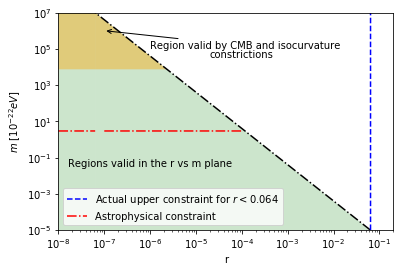
\includegraphics[width=8cm]{SFDMconstraints.png}
\caption{Isocurvature constraints for the SFDM candidate.
\jav{ya me confundio esta figura. Seria bueno poner los ejes al reves, ya que $r$ se esta buscando 
y $m$ seria un derivado. De acuerdo a esta figura, cuales son las constricciones actuales a la masa?}
\jav{quitar la flecha y mejor centrar el texto, explicar regiones.}
}\label{constraintsSFDM}
\end{figure}

%%%-------------------------------------------------------------------------------------------%%%
\subsubsection{Self-interacting SFDM scenario} 
%%%-------------------------------------------------------------------------------------------%%%

When the massive SFDM scenario is compared with observations there exist 
several discrepancies about the constrictions of the mass. 
For example when the model is tested at galactic levels, by considering that its ground state of the self-gravitating 
BEC corresponds to the minimum DM halo, it is obtained a mass $m=2.92\times 10^{-22}eV$ \jav{exactamente igual?}
\cite{massconst1,SFphi42};
 if on the other hand the massive model is tested at cosmological levels considering big bang 
 nucleosynthesis (BBN) constraints, it is obtained that $m>7.38\times 10^{-19}eV$ (see \cite{SFphi41,SFphi42}), 
 which is clearly a disagreement with the constraints given by galactic scales. 
 For this reason is convenient to extend the model and introduce a self-interacting term that can help us to relax these discrepancies. 
 \jav{esta expliacion deberia ir antes de la ecuacion (38), donde por primera vez menciones $\psi^4$, o inclusive en la introduccion.}
 For simplicity we continue considering that the SF does not interact with the inflaton 
 in such case the total potential of the system can be given by \jav{es la misma que la eqn (39)}
 %
\begin{equation}
V(\phi,|\psi|^2)=V(\phi)+\frac{1}{2}m^2\psi^2+\frac{1}{4}\lambda\psi^4.
\end{equation}
%

As we have shown in the last section we have 2 different scenarios for this model: 
a weak interacting and a strong interacting. In the weak interacting model our SFDM behaves 
effectively as a massive field without auto-interaction, and in such case the constrictions 
for the massive field applies to this scenario too. On the other hand when the auto-interacting 
term is big enough, the SFDM will have a new period with behavior of radiation-like fluid. 
In this way the constrictions we obtained before will not apply to this model anymore \jav{por que?}
\jav{osea que el weak interacting, no aporta nada?}.

%Before studying the strong scenario notice that we can give general constrictions for the 
%auto-interacting contribution in terms of our previous expressions. 
As we observed in the last section 
we have the weakly self-interacting regime when $m^2\gg \lambda|\psi_i|^2/2$. In fact, thanks to the 
decreasing behavior of these scenarios we can consider that this regime is fulfilled always that 
$m^2\geq \lambda|\psi_i|^2/2$ or equivalently when $\lambda\leq 2m^2/|\psi_i|^2$. 
%
If the SFDM oscillations start at the same time than the massive case (which is a good approximation), 
\jav{por que es una buena aproximacion?}
we observe from \eqref{phi_im2} that constrictions can be given in terms of the mass $m$ of the SF as
%
\begin{equation}
\left(\frac{\lambda}{10^{-96}}\right)\leq 1.2\left(\frac{m}{10^{-22}eV}\right)^{5/2}.
\end{equation}
%\jav{estamos hablando del strong or weakly scenario? porq la ecuacion que usas se basa en el weakly scenario!!} 
\jav{tal vez juntar esta parte con la del section iii, de self-interacting scalar field.}
We plot in figure \ref{weekregime} the weak limit obtained by our approximation. 
However this overestimates the value of $\lambda$ since in the above expression we have an 
equality the field is not behaved as a dust-like field at all, 
this behavior is obtained when the $\lambda$ term is completely negligible.
\jav{reacomodar y reescribir. Esto va junto con el weakly scenario.}
%
\begin{figure}
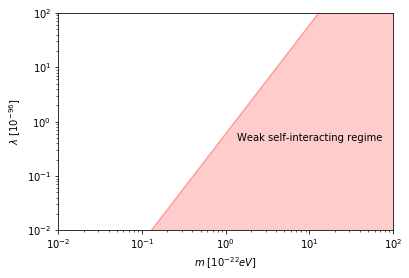
\includegraphics[width=8cm]{weakregime.png}
\caption{Weakly self-interacting regime, \jav{explicar regiones, quitar flecha y mejor centrar el texto}}
\label{weekregime}
\end{figure} 

In the strong self-interacting regime, during the inflationary era, the SFDM follows the attractor solution \eqref{atractor}.
%\begin{equation}\label{atractor0}
%\psi_{att} =\left(2\lambda\int_{\phi}^{\phi_0}V^{-1}_{,\phi}d\phi\right)^{-1/2}
%\end{equation}
The value that the homogeneous field acquired  after inflation depends on the condition 
$\psi_{att}<\sqrt{2}m/\sqrt{\lambda}\equiv \psi_t$. 
For $\psi_{att}<\psi_t$ the field follows the attractor solution until $\psi\simeq \psi_t$. 
Then the scalar field is frozen at that value and starts oscillating as a massive field 
when $m\sim H$. Notice that we can do two kind of constrictions of our free parameters in this scenario. 
First, from equation \eqref{initial_c} and taking $\psi_i=\psi_t$ we have
%
\begin{equation}
r<1.2\times 10^{-4}\left[\frac{\left(\frac{m}{10^{-22}eV}\right)^2}{\frac{\lambda}{10^{-96}}}\right].
\end{equation}
%
While thanks to the fact that when the SFDM starts its oscillations it behaves as a massive field, 
the constrictions obtained in the non-interacting field must be fulfilled as well. 
Matching $\psi_t$ with \eqref{phi_im2} and considering the constriction given by the 
primordial tensor perturbations (eq. \eqref{constm}) we obtain
%
\begin{equation}
\left(\frac{\lambda}{10^{-96}}\right)\leq 1.2\left(\frac{2\times 10^{-4}}{r}\right)^5.
\end{equation}
In figure \ref{constraintsSFDMl} we have plotted the above condition that is valid in the weak \jav{weak? sure? al inicio del parrafo 
dice strong}  interacting regime.

\begin{figure}[h]
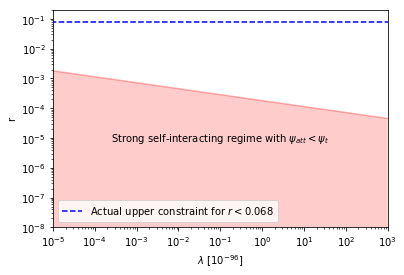
\includegraphics[width=8cm]{lambdavsr.png}
\caption{Isocurvature constraints for the weakly self-interacting term. \jav{weak?}}\label{constraintsSFDMl}
\end{figure} 

Additionally, in this scenario, the inflationary potential fulfills the condition 
%
\begin{equation}
\left(\int^{\phi_0}_\phi V_{,\phi}^{-1}d\phi\right)^{-1/2}<2m.
\end{equation}
%
We can see that it is very difficult to obtain this relation for an ultra-light SFDM candidate. 
For example, if we consider a chaotic-like inflationary potential, $V(\phi)=\frac{1}{2}M_{inf}^2\phi^2$, 
the above conditions implies that
%
\begin{equation}\label{chaoticweek}
\left(\log\frac{\phi_0}{\phi}\right)^{-1/2}<2\frac{m}{M_{inf}}.
\end{equation}
%
However, in a chaotic-like inflationary potential the mass $M_{inf}$ of the inflaton 
that best matches the observations\footnote{This chaotic-like inflationary potential is 
ruled-out now for observations, however we use it as an example in order to obtain 
general constraints for our models.} is of order $M_{inf}\sim 10^{12} GeV$ \cite{Liddle}. 
If now we assume an ultra-light SFDM candidate with a mass $m\sim 10^{-22}eV$, 
the above conditions implies that the logarithmic part of the expression should be 
lower that $\sim 10^{-43}$. The inflationary behavior for a chaotic-like inflaton ends 
when $\phi_{end}\simeq 2M_{pl}$ \cite{curvatonatractor,Liddle}. Moreover as it is 
explained in \cite{curvatonatractor}, the initial condition of the inflaton cannot be 
arbitrarily large since the stochastic behavior is significant for $\dot\phi H^{-1}<H/2\pi$. 
%
If the Universe starts when the inflaton escapes from the stochastic 
behavior we have that the initial condition  should be
%
\begin{equation}\label{phi_0}
\phi_0\sim 10^5\times M_{pl}\left(\frac{10^{13}GeV}{M_{inf}}\right)^{1/2}.
\end{equation}
%
where we can easily see that the condition given in \eqref{chaoticweek} cannot be fulfilled 
\jav{y si no se satisface, que pasa?}.

When $\psi_{att}>\psi_t$ we have that the field follows the attractor solution during all the period of inflation. 
In this way the initial condition for the SFDM  given by \eqref{atractor2}
%
\begin{equation}\label{atractor3}
\psi_{att}^i = \left(2\lambda\int_{\phi_{end}}^{\phi_0}V^{-1}_{,\phi}d\phi\right)^{-1/2}.
\end{equation}
%
Then the SFDM remains frozen at value $\psi_{att}^i$ until $M\sim H$ and starts oscillating with a 
quartic potential. In this scenario the SF density behaves as $\rho_{SFDM}\propto \psi^4$ and 
in such case we can write $P_{SFDM}=4\delta\psi/\psi_i$. In this way the primordial 
isocurvature perturbations for a strong-interacting SFDM is given by
%
\begin{equation}
P_{SFDM}(k)=\left(\frac{2H_*}{\pi\psi_i}\right)^2.
\end{equation}
%
In the last section we showed the relation of the initial condition  with the value of the 
field today. Using eqs. \eqref{inilamb2} and \eqref{phi_im2}, 
with $g_{*osc}=3.36$ and $g_{s*osc}=3.91$  and considering the appropriate units,  
similar to the ones obtained in \eqref{initial_c}, we obtain
%
\begin{equation}\label{constr4}
r<\frac{1.172\times 10^{-4}}{7^{1/3}f^2(\sigma)}\left[\frac{2
\left(\frac{m}{10^{-22}eV}\right)^{3/2}}{\left(\frac{\lambda}{10^{-96}}\right)}\right]^{1/2}.
\end{equation}
%
We show in figure \ref{constraintsSFDMls} constraints obtained for the strong scenario 
in terms of tensor-to-scalar ratio. 
We plotted contours of the value of the right side on the above equation \jav{ser mas especifico}. 
Notice that the gray region in the figure corresponds with values larger that $0.08$ 
which are the current upper limit for $r$. This implies that such region is already allowed by the model. 
It is necessary to mention that there are some region of parameters where the strong and 
the weakly scenarios are overlapped in our approximations \jav{cuales? mostrar}. This is because the 
simplifications  we had in our analysis \jav{es bueno, malo?}. 
However these descriptions can give us general considerations for our SFDM models. 
Figure \jav{[?]} shows that as long as the mass parameter $m$ of the SF decreases, 
the possible values of the auto-interacting parameter is less restrictive. On the other hand we observe 
that if we fix a mass $m$, it is possible to avoid isocurvature perturbations by increasing the value of 
the auto-interacting term. 
For example, let us suppose that we are interested in a model with a mass $m\sim 10^{-21} eV$ in the strong regime. 
Let us assume as well that future experiments on gravitational waves measure $r\sim 0.05,0.01,0.001$. 
In this way we obtain from figure \ref{constraintsSFDMls} that such observations should imply 
that $\lambda>10^{-94},10^{-95},10^{-97}$, where the last constriction is obtained by the 
lower value for $\lambda$ in the strong scenario.   \jav{explicar colores, regiones, ejes, etc..}
%
\begin{figure}
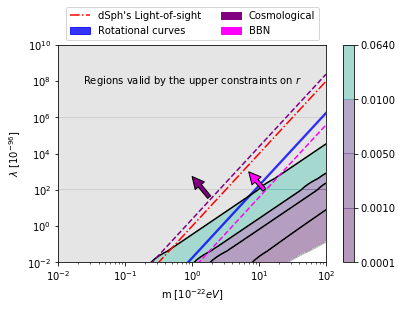
\includegraphics[width=8cm]{stronglamb.png}
\caption{Isocurvature constraints for the strong auto-interacting scenario.
\jav{explicar bien}}\label{constraintsSFDMls}
\end{figure} 

Remark: This scenario is of special interest given that the attractor solution justify the initial 
conditions for the SFDM model and because it is natural to avoid isocurvature perturbations 
when the auto-interacting term of the SF is big enough.
 
\jav{aqui me quede}
Similarly to the above description we can do general constraints for the inflationary 
potential that should generate inflation on these kind of scenarios. First we have that
%
\begin{equation}
\left(\int^{\phi_0}_\phi V_{,\phi}^{-1}d\phi\right)^{-1/2}>2m,
\end{equation}
which is very easy to fulfilled as we saw in the chaotic-like example. 
This relation can be translated into constrictions in the tensor-to-scalar ratio as
\begin{equation}
r<\frac{0.6\times 10^{40}}{\left(\frac{\lambda}{10^{-96}}\right)}\left(\frac{1}{\int_{\phi_{end}}^{\phi_0}V_{,\phi}^{-1}d\phi}\right),
\end{equation}
that can also be easily fulfilled always that the auto-interacting term and the integral are not extremely big; for example in the chaotic-like scenario by using \eqref{chaoticweek} and \eqref{phi_0}
%\begin{equation}
%\left(\int^{\phi_0}_\phi V_{,\phi}^{-1}d\phi\right)^{-1/2}\simeq (0.7403)\times 10^{21}
%\end{equation}
and taking $M_{inf}\simeq 10^{-6}M_{pl} $, we can obtain the constriction \textcolor{red}{No entend\'i aqu\'i que debo cambiar}
\begin{equation}
\left(\frac{\lambda}{10^{-96}}\right)<\frac{0.3288\times 10^{84}}{r}.
\end{equation}
If now we compare \eqref{atractor2} and \eqref{inilamb2} we have
\begin{equation}\label{inilamb3}
\left(\int_{\phi_{end}}^{\phi_0}V^{-1}_{,\phi}d\phi\right)^{-1}=\frac{6}{7^{1/3}f^2(\sigma)}\left(2m^2\lambda|\psi_t|^2\right)^{1/2}.
\end{equation}
This relation can be interpreted as follows: consider that we are interested in an auto-interacting SFDM candidate that coexist with the inflaton. Suppose we have several measurements that constraints the mass parameter $m$ of the model as well as the auto-interacting one. In this way we can see that such constraints can be translated into constraints to the inflationary potential that causes inflation.  

It is also necessary to be careful that the SFDM does not come to dominate the inflationary period.  This is guarantee by demanding that
\begin{equation}
\lambda < \frac{H_*^2 M_p^2}{|\psi_i|^4}.
\end{equation}
Or in terms of \eqref{atractor3}
\begin{equation}
\lambda>\left(4H_*^2M_{pl}^2\left(\int_{\phi_{end}}^{\phi_0}V_{,\phi}^{-1}d\phi\right)^2\right)^{-1}.
\end{equation}
Considering again the chaotic-like example and using $H_*= 10^{14} GeV$, we obain the constriction
\begin{equation}\label{lowerlambda}
\frac{\lambda}{10^{-96}} > 5.777\times 10^{77}.
\end{equation}
\begin{center}
\textit{Complex SFDM generalization}
\end{center}
% A massive complex scalar field is described by the potential
%\begin{equation}
%V(|\psi|^2)= m^2|\psi|^2
%\end{equation}
As we have shown in last section when we consider a complex scalar field its dynamics is modified only by the centrifugal term (see eq. \eqref{KGe3}). However as it was mentioned in \cite{SFphi42} such term does not affect the dynamics of the field at cosmological levels, obtaining then that a complex scalar field and a real scalar field have the same cosmological history in the Universe. In this way if we consider that our complex SFDM fulfilled slow-roll conditions during inflation its constrictions for isocurvature perturbations must be the same than in the real field analogue. \\
\begin{center}
\textit{Different constraints for the self-interacting SFDM model}
\end{center}

This auto-interacting model can be tested at galactical levels by considering that its ground state corresponds with the minimum galaxy halo (Fornax) \cite{SFphi42}. With such observations we can constraint the ratio $\lambda/m^2$. If additionally we use constraints obtained by the Bullet Cluster \cite{bullet} it is possible to set the free parameters of the model. In \cite{SFphi42} it was obtained that for a strong self-interacting SFDM model we have
\begin{equation}
m= 1.10\times10^{-3}eV, \ \ \ \ \lambda = 2.46\times 10^{-17},
\end{equation}
while for a week self-interacting model we obtain
\begin{equation}
m= 2.92\times 10^{-22}eV.
\end{equation}
This results corresponds with lower and upper bounds of the mass of the SFDM. In this way the mass of the SFDM should be in the range $2.92\times 10^{-22}\leq m\leq 1.10\times 10^{-3}eV$.

On the other hand when the model is tested at cosmological levels using the CMB and the abundances of ight elements produced by the BBN it is obtained the values \cite{SFphi41,SFphi42}
\begin{equation}\label{masslamb}
m=3\times 10^{-21}eV, \ \ \ \ \ \lambda = 1.69\times 10^{-87}.
\end{equation}
Notice that these last expressions are in agreement with the ones given by galactic constrictions.

Considering \eqref{masslamb} as the most acceptable values for the mass of the SFDM and its auto-interacting term we can easily see from figure \ref{weekregime} that we should be in the strong regime. Then in this scenario the constrictions given in Eq. \eqref{constr4} (or equivalentily in figure \ref{constraintsSFDMls}) should apply. We observe in figure \ref{constraintsSFDMls} that the parameters obtained by BBN are easily acepted by the model due to the fact that those parameters are in the region that are already completely allowed by the constraints in the measurement on tensor-to-scalar ratio (grey region on the figure) which implies that the isocurvature perturbations are small enough that can avoid actual upper restrictions. In this way isocurvature perturbations does not represent any problem for the autointeracting model that matches with cosmological and galactical constrictions.

Observe that these parameters do not match with the lower constraints obtained in \eqref{lowerlambda}. This are not a problem for auto-interacting SFDM models since Eq. \eqref{lowerlambda} is obtained for a chaotic-like inflationary potential and, as we already know, that inflationary model is ruled-out by the actual constraints given by Planck \cite{planck}.

\section{Another idea/paper}
\subsection{Comments on Curvaton scenarios}

In the curvaton scenario it is assumed that during inflation there was an extra scalar field that coexist with the inflaton and its classical dynamics was negligible (its energy density was sub-dominant during inflation). Then, similar to the SFDM scenario, this SF obtained quantum fluctuations. If the curvaton field is long lived (at least its life must be longer than the inflaton one) it starts to oscillate when the Hubble scale $H$ approaches the curvaton mass shortly before or after the inflaton decays to radiation. During its oscillation phase, this curvaton field starts to behave as dust and then its energy density decreases slower than the ones associated with the inflaton (see appendix [B] for a review of the model). If the curvaton decays to radiation when its quantum fluctuations dominate over the inflaton ones, we can obtain a scenario where curvaton quantum fluctuations can dominate the early Universe and give place to be the totality of the initial adiabatic perturbations. In the formalism showed in \ref{Generalities} and as it is explained in \cite{twofields}, such scenario is obtained when $T_{RS}>>1$ or equivalently when we consider in our analysis $\sin\Delta = 0$, in such case we obtain that the tensor-to-scalar ratio in the pure curvaton scenario is $r=0$. 

There is also generation of isocurvature fluctuations on this scenario given by equation \eqref{PsAs}. Such fluctuations can be generated always that the DM or baryons were generated before the decay of the curvaton or for the decay products of the curvaton \cite{curvaton9,curvaton10,curvaton11}. To be precise depending on how various particle numbers were generated they will inherit the curvaton, the inflaton or the total curvature fluctuations. For example, following \cite{curv2,curvaton11,curvaton14}, if the baryons or DM were created before the curvaton decays then they inherit inflaton's fluctuations, $P_R^\psi$. If they were generated by curvaton decays, they inherit the curvaton's fluctuations, $P_R^\sigma$. If they were generated before the curvaton decays they inherit the total curvature perturbation $P_R$. If they were generated after curvaton decays, isocurvature perturbations are not produced. There are other possibilities where one of the components were generated after curvaton decays and the other by, in such case every fluid inherit a different curvature perturbation, or the possibilty that compensated isocurvature perturbations \cite{curvaton14} were generated by all the processes mentioned before. Depending on the momment when baryons and DM were generated we will have several scenarios that can fulfill actual constraints or not (see table I of reference \cite{curvaton14}). In this section and in order to simplify our analysis, we consider that we are already in a scenario where isocurvature perturbations satisfies observations. We also demmand that the total inflationary potential can be written as $V(\psi,\sigma)=V(\psi)+V(\sigma)$ wich implies that the fields are not correlated and then correlated fluctuations \eqref{PrCrs} are not generated. 

In the last few years researchers have started to study curvaton models but considering that the curvaton field does not constribute to the totality of the primordial adiabatic perturbations, instead, it contributes to a fraction of them, while the remaining one is produced by the inflaton \cite{curvaton4,curvaton5,curvaton6,curvaton7,curvaton8} (or for a more resent study see \cite{curvaton3}). This scenario is the so-called \textit{mixed inflationary model}. Notice that such scenario is obtained if $0<\cos\Delta <1$. It is also usual to redefine a new parameter in this model $\hat R= [\cot^2\Delta]_{k_0}$ which can be related with the curvaton-to-inflaton density fraction of primordial curvature perturbations. Then, the primordial curvature perturbations can be written from \eqref{PrAs} as
\begin{equation}\label{PCr}
\mathcal{P}_R(k)=A_r\left(\left(\frac{k}{k_{0}}\right)^{n_s^\phi-1}+\hat R\left(\frac{k}{k_{0}}\right)^{n_s^\sigma-1}\right),
\end{equation}
where $n_s^\phi-1 = -6\epsilon_\phi+2\psi_{\phi\phi}$ and $n_s^\sigma-1 = -2\epsilon_\sigma+2\psi_{\sigma\sigma}$.
The total spectral index ($n_s-1=d\ln P_R/d\ln k$) is given then by
\begin{equation}
n_s-1=\frac{n_s^\phi+\hat R n_s^\sigma}{1+\hat R}-1.
\end{equation}
From \eqref{Tensortoscalar} the tensor-to-scalar ratio in this model is given by
\begin{equation}\label{tensortoscalar}
r=\frac{16\epsilon_\phi}{1+\hat R}.
\end{equation}		
We can notice then that depending on the value of $\hat R$ we can obtain different values for the inflationary observables. When $\hat R=0$ we obtain the inflation scenario, whereas if $\hat R\gg 1$ we obtain the pure curvaton scenario.  

The possible values that $\hat R$ can obtain depend on the particular model of inflation, the value that the curvaton had during inflation and its evolution history (see appendix [B] and equation \eqref{R_r}). In particular it depends linearly on $\epsilon_\psi$, which implies that the larger $\epsilon_\psi$ is, the larger the curvaton contribution. For example, for large field inflationary models the curvaton can contribute more to the primordial curvature perturbations, while for small field models, the curvaton contributes less. This result is very convenint because large-field models usually predict large tensor-to-scalar ratio observations, while last observations allow small $r$ \eqref{Tensortoscalar}. In this way we notice that the addition of a new free parameter can help to relax different inflationary models.  

In \cite{curvaton15} it was studied chaotic-like inflationary models with an extra light scalar field. In such study it was obtained that one of the most preferable scenarios is a quartic-like inflationary potential with our extra scalar spectator. However it is necessary to notice that such scenario is favorable only when the mass of the curvaton is negligible compared with the Hubble parameter. For the main purpose of this article we take that example and observe how the inflationary parameters are predicted by the model. In fact when we consider the chaotic potential $V(\phi)=(1/2)\lambda_p\phi^p$ for the inflaton and the  potential $V(\sigma)= (1/2)M^2\sigma^2$ for the curvaton, the spectral index $n_s$ is rewritten as
\begin{equation}
\label{nsexplicit}
n_s-1\approx -\frac{1}{1+\hat R}\frac{2(2+p)}{4N+p}+\frac{\hat R}{1+\hat R}\left[-\frac{2p}{4N+p}+\frac{2M^2}{3H_*^2}\right],
\end{equation}
where  $N$ is the number of e-folds produced before our scales left the horizon and it is usually used $N=50\sim 60$. In the above equation we have used the Friedman equation in the slow-roll approximation for the term containing $M$. If we use \eqref{tensortoscalar} into \eqref{nsexplicit} we have 
\begin{equation}
n_s-1=-\frac{(2+p)}{8p}r+\left[1-\frac{(4N+p)}{16p}r\right]\left[\frac{2}{3}\frac{M^2}{H^2}-\frac{2p}{4N+p}\right],
\end{equation}
where we have obtained a relation between the spectral index and the tensor-to-scalar ratio which are well constrain by the data. Notice that in the limit when the curvaton dominates completely the adiabatic perturbations ($r\simeq 0$) and considering the mass of the curvaton negligible compared with the Hubble parameter (i.e. $M<<H$) we obtain that $n_s-1\simeq p/(120+p/2)$ and then the observational constrains for the spectral index \eqref{n_R} means that the inflaton field must be close to be a quartic potential, $p=4$. Such result can be observed in figure \ref{nvsr}, where we have plotted the above equation neglecting $M/H$. In such figure we can observe an upper an lower value for $n_s$ in terms of $r$ which is obtained when we consider $N=60-50$ e-folds at the moment when our scales left the horizon. On the other hand we could consider the next level of complication allowing $M/H$ to vary using as our constriction that $M/H<1$ (in order to obtain quantum fluctuations for the curvaton during inflation), considering that the curvaton never dominates during the inflationary era, which is guarantied when
\begin{equation}\label{MoverH}
\frac{M^2}{H^2_*}<\frac{M_{pl}^2}{\sigma_i^2},
\end{equation} 
and that its oscillations starts after inflaton oscillations, which implies
\begin{equation}\label{M2curv}
M^2\lesssim p(p-1)\lambda_p \psi_{end}^{p-2},
\end{equation}
where $\psi_{end}$ is the value of $\psi$ at the end of inflation. We can see from \eqref{R_r} that $(M_{pl}^2/\sigma_i^2)\sim R/\epsilon r_{dec}^2$. In a typical scenario $r_{dec}^2\ll 1$, while $\epsilon\ll 1$ by slow-roll construction. Then, if we allow $\hat R$ to be big enough (we are not in the just inflationary scenario) expression \eqref{MoverH} is fulfilled trivially when we demmand $M/H<1$. Inflaton oscillations starts inmediatelly after inflations ends, then we take that $0<M^2/H^2<1$. In figures \ref{curv50} and \ref{curv60} we have plotted contour regions for $r$ in the plane $M^2/H^2\ vs\ n_s$ in the range $10^{-5}<M^2/H_*^2<0.5$, for $N=50,60$ and for $p=1,2,3,4,5,6$. As we can see when only $r$ and $n_s$ are consider it looks that quartic and cubic potentials can fit well observations. For the typical quadratic and the linear potentials we can see that we can obtain parameters that are inside actual bonds on the parameters but only by obtaining relatively large $r$. For the last two potentials it is also possible to obtain the observations required but only when $M/H$ is not so small and for a very little region of parameters.   
\begin{figure}
\centering
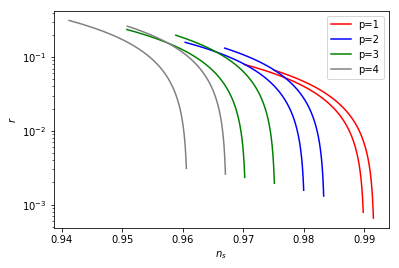
\includegraphics[width=0.4\textwidth]{nvsr}
\caption{Possible values in the n vs r plane when we allow $R$ to vary. The values that can be produced by the models are the ones between the two limits plotted in the figure.\textcolor{red}{(Tratar de pintar las regiones entre las l\'ineas y poner los datos de Planck para que se vea mejor.)}}
\label{nvsr}
\end{figure}
% * <epadilla@fis.cinvestav.mx> 2018-04-29T03:33:02.572Z:
%
% ^.
\begin{figure}[h!]
\raggedright
\begin{subfigure}[b]{0.6\textwidth}
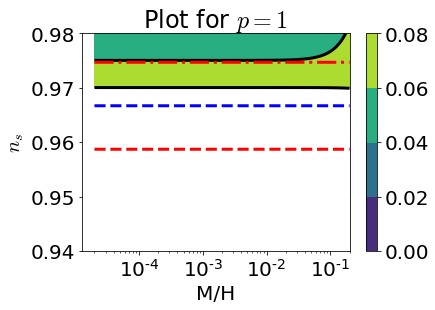
\includegraphics[width=0.3\textwidth]{p150.png}
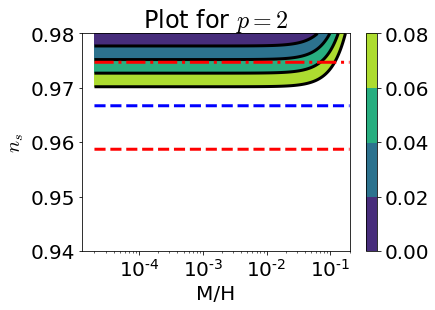
\includegraphics[width=0.3\textwidth]{p250.png}\\
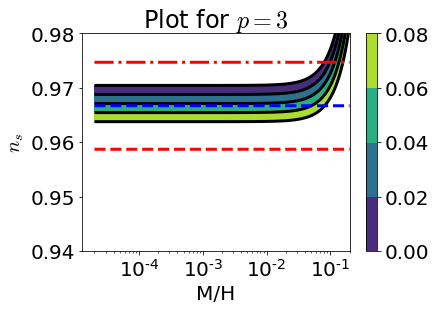
\includegraphics[width=0.3\textwidth]{p350.png}
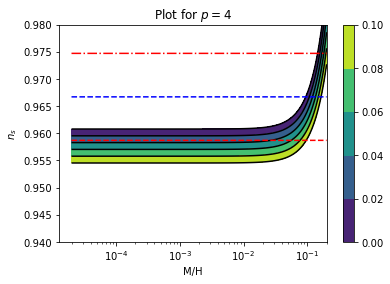
\includegraphics[width=0.3\textwidth]{p450.png}\\
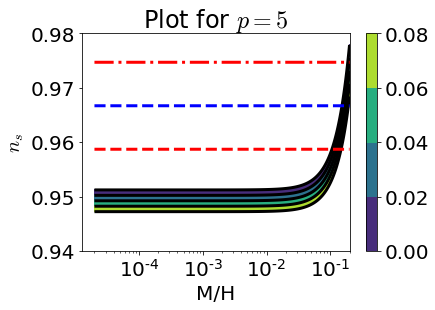
\includegraphics[width=0.3\textwidth]{p550.png}
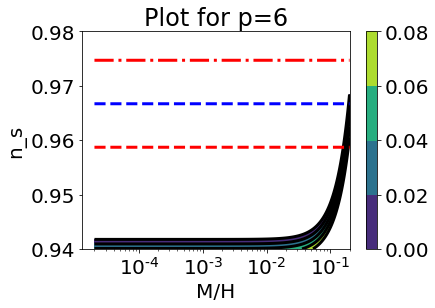
\includegraphics[width=0.3\textwidth]{p650.png}
\end{subfigure}
\caption{Inflationary constraints in the $M/H$ vs $n_s$ plane for $N=50$ e-folds. We plotted contour regions for $0<r<0.1$.}
\label{curv50}
\begin{subfigure}[b]{0.6\textwidth}
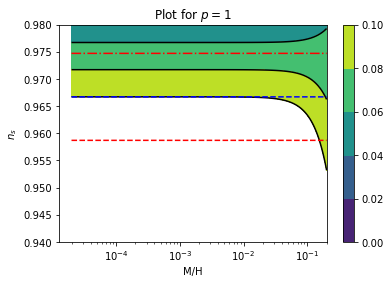
\includegraphics[width=0.3\textwidth]{p160.png}
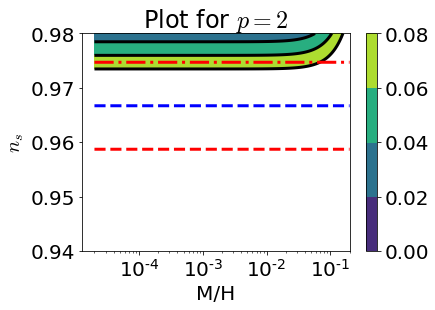
\includegraphics[width=0.3\textwidth]{p260.png}\\ 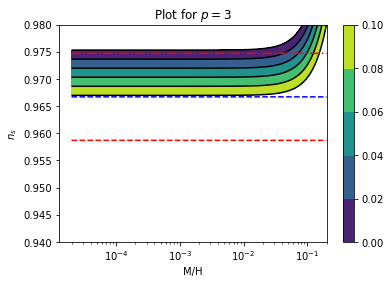
\includegraphics[width=0.3\textwidth]{p360.png}
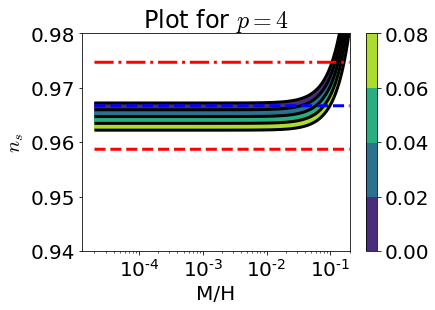
\includegraphics[width=0.3\textwidth]{p460.png}\\
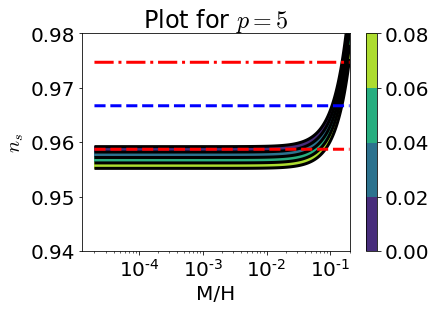
\includegraphics[width=0.3\textwidth]{p560.png}
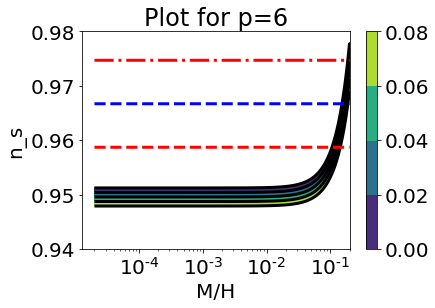
\includegraphics[width=0.3\textwidth]{p660.png}
%\captionof{figure}
%{\footnotesize{A }}
\end{subfigure}
\caption{Inflationary constraints in the $M/H$ vs $n_s$ plane for $N=60$ e-folds. We plotted contour regions for $0<r<0.1$.}\label{curv60}

\end{figure}
\subsection{Constraining curvaton models with last data}
\textcolor{red}{(Esta ser\'ia tu parte, Beto)}
\section{Conclusions}\label{conclusions}
\appendix
\section{Slow-Roll index}

In this appendix we define the slow roll indexes used in our calculation. We have:
\begin{subequations}
\begin{equation}
\epsilon_i = \frac{1}{16 \pi G}\left(\frac{V_i}{V}\right)^2, \ \ \ \ \ \text{where $i=\phi,\psi$},
\end{equation}
\begin{equation}
\psi_{ij}=\frac{1}{8\pi G}\left(\frac{V_{ij}}{V}\right),
\end{equation}
\end{subequations}
where $V_i = \partial V/\partial \phi_i$. In the other side we have
\begin{equation}
\epsilon \equiv \frac{1}{16\pi G}\left(\frac{V_\sigma}{V}\right)^2\simeq \epsilon_\phi+\epsilon_\psi,
\end{equation}
and
\begin{eqnarray}
\eta_{\sigma\sigma}&=&\eta_{\phi\phi}\cos^2\theta + 2\eta_{\phi\psi}\cos\theta\sin\theta+\eta_{\psi\psi}\sin^2\theta\nonumber \\
\eta_{\sigma s}&=&(\eta_{\psi\psi}-\eta_{\phi\phi})\sin\theta\cos\theta + \eta_{\phi\psi}(\cos^2\theta-\sin^2\theta)\\
\eta_{ss}&=&\eta_{\phi\phi}\sin^2\theta - 2\eta_{\phi\psi}\cos\theta\sin\theta+\eta_{\psi\psi}\cos^2\theta\nonumber .
\end{eqnarray}
\section{A review on the physics on Curvaton models}

The curvaton $\sigma$\footnote{We use $\sigma$ since it is the most commun way that the curvaton field is represented in literature} is a real light scalar field during inflation which starts to oscilate when the Hubble parameter approaches to its mass $m_\sigma$ shortly before or after the inflaton $\phi$ decays into radiation. It was propossed in \cite{curvaton1,curv2,curv3} as an alternative mechanism for generating the primordial density perturbation on the Universe. In the typical scenario the curvaton is assumed to be quadratic on its potential which implies that when its oscillations starts it behaves as a pressureless fluid. During its oscillation phase and considering that the inflaton has already decay we have that bouth fluids evolves as $\rho_\sigma\sim a^{-3}$ (dust-like evolution) an $\rho_{rad}\sim a^{-4}$ (radiation-like evolution). In this way we can see that during this period the curvaton energy density decreases slower than the inflaton one and then its fraction contribution for the total energy of the Universe can be larger and larger and generate curvature fluctuations \cite{curvaton1,curv2,curv3}.

In this scenario, the curvature perturbation $R$ evolves until the curvaton decays. Then $R$ stops evolving and becomes constant at the super-horizon scale. In the general scenario both fluids can be responsabble for the generation of the primordial curvature fluctuation $R$. If we assume that $\phi$ and $\sigma$ are uncorrelated, the power spectrum of curvature perturbations $P_R$ is given by
\begin{subequations}
\begin{equation}
P_R(k)=P_R^{(\phi)}(k)+P_R^{(\sigma)}(k)=(1+\hat R)P_R^{(\phi)},
\end{equation}
where $P_R^{(\phi,\sigma)}$ are the power spectra for the curvature perturbation generated by the field $\phi,\ \sigma$ and we have defined the ratio $\hat R$ between bout spetra as
\begin{equation}
\hat R\equiv \frac{P_R^{(\sigma)}}{P_R^{(\phi)}}.
\end{equation}
\end{subequations}
The fraction $\hat R$ can be also related with the ratio $r_{dec}$ of curvaton energy $\rho_\sigma$ to radiation energy $\rho_{rad}$  at the time of the curvaton decay as
\begin{equation}\label{R_r}
\hat R =\frac{8}{9}\epsilon \left(\frac{M_{pl}}{\sigma_i}\right)^2 r^2_{dec},
\end{equation}
where $\sigma_i$ is the value of the curvaton during inflation and
\begin{equation}
r_{dec} =\left.\frac{\rho_\sigma}{\rho_\sigma + 4\rho_{rad}/3}\right|_{dec}.
\end{equation}
Notice that the pure curvaton senario is obtained when $ R\gg 1$ and then the primordial curvature perturbations are generated only by $\sigma$.

When the curvaton decays and considering that the Universe is domminated by a radion-dominated era, $r_{dec}$ can be approximated as \cite{curv2,curvaton3}
\begin{equation}
r_{dec}\sim \left(\frac{\sigma_*}{M_{pl}}\right)^2\sqrt{\frac{m_\sigma}{\Gamma_{\sigma}}},
\end{equation}
where $\Gamma_\sigma$ is the decay rate for the curvaton.
%\section{Papers} 
%Aqu\'i pondré de mientras los links de los papers que he revisado:

%https://arxiv.org/pdf/1211.3535.pdf

%https://arxiv.org/pdf/1712.05364.pdf

%https://arxiv.org/pdf/1505.00639.pdf

%https://arxiv.org/pdf/astro-ph/0306500.pdf

%https://arxiv.org/pdf/1708.05681.pdf

%https://arxiv.org/pdf/1211.3535.pdf

%https://arxiv.org/pdf/1507.00119.pdf

%https://arxiv.org/pdf/1801.07409.pdf

%https://arxiv.org/pdf/1305.5338.pdf

\begin{thebibliography}{9}
\bibitem{const1}  P. A. R. Ade
et al.
(Planck), Astron. Astrophys.
571
, A16 (2014), arXiv:1303.5076 [astro-
ph.CO]
\bibitem{const2} ]  P. A. R. Ade
et al.
(Planck), Astron. Astrophys.
571
, A22 (2014), arXiv:1303.5082 [astro-
ph.CO]
\bibitem{planck} P. A. R. Ade et al. (Planck); DOI: 	10.1051/0004-6361/201525898;  	arXiv:1502.02114 [astro-ph.CO]
\bibitem{SF1} Baldeschi M., Gelmini G., Ruffini R., 1983, Phys.Lett.B, 12
\bibitem{SF2} Matos T., Guzman F. S., 2000, Class. Quant. Grav. 
\bibitem{SF3} Hu W., Barkana R., Gruzinov A., 2000, Physical Review Letters, 85, 1158
\bibitem{SF4}Bray H., 2010
\bibitem{SF5}Schive H.-Y., Chiueh T., Broadhurst T., 2014a, Nature Phys., 10, 496
\bibitem{SF6}B\"ohmer C. G., Harko T., 2007, J. Cosmology Astropart. Phys., 6, 025
\bibitem{SF7}Marsh D. J. E., Ferreira P. G., 2010, Phys. Rev. D, 82, 103528
\bibitem{SF8} Membrado M., Pacheco A. F., Sa\~nudo J., 1989, Phys.Rev.A, 39, 4207
\bibitem{LCDM1}Peebles P. J. E., 1982, ApJ, 263, L1.
\bibitem{LCDM2}White S. D. M., Frenk C. S., Davis M. et al., 1987, ApJ, 313, 505.
\bibitem{problem1}Bullock J. S., Boylan-Kolchin M., 2017, ARA$\&$A, 55, 343
\bibitem{problem2}Clowe D., Bradac M., Gonzalez A. H. et al., 2006, ApJ, 648, 2.
\bibitem{problem3}Klypin A., Kravtsov A. V., Valenzuela O. et al., 1999, ApJ, 522, 82.
\bibitem{problem4}Moore B., Ghigna S., Governato F. et al., 1999, ApJ, 524, L19.
\bibitem{problem5}Penny S., Conselice C. J., De Rijcke S. et al., 2009, MNRAS, 393, 1054.
\bibitem{SF9} J. Maga\~na and T. Matos,  Journal of Physics: Conference Series, Volume 378, conference 1
\bibitem{SF10}  A. Su\'arez, V. H. Robles, and T. Matos, Astrophys. Space
Sci. Proc.
38
, 107 (2014), 1302.0903.
\bibitem{SF11} Marsh D. J. E., 2016, Phys. Rep., 643, 1
\bibitem{SF12}  L. Hui, J. P. Ostriker, S. Tremaine, and E. Witten, Phys. Rev. D
95
, 043541 (2017).
\bibitem{curv1}K. Enqvist and M. S. Sloth, Nucl. Phys. B
626
(2002) 395 doi:10.1016/S0550-3213(02)00043-3
[hep-ph/0109214
\bibitem{curv2} D. H. Lyth and D. Wands, Phys. Lett. B
524
(2002) 5 doi:10.1016/S0370-2693(01)01366-1
[hep-ph/0110002
\bibitem{curv3} T. Moroi and T. Takahashi, Phys. Lett. B
522
(2001) 215 [hep-ph/0110096]
\bibitem{twofields} Christian T. Byrnes, David Wands;  Phys.Rev. D74 (2006) 043529; DOI:  	10.1103/PhysRevD.74.043529;  arXiv:astro-ph/0605679v3
\bibitem{const3}  D. Barkats
et al.
(BICEP1), Astrophys. J.
783
, 67 (2014), arXiv:1310.1422 [astro-ph.C]
\bibitem{const4} P. A. R. Ade
et al.
(BICEP2, Planck), Phys. Rev. Lett.
114
, 101301 (2015), arXiv:1502.00612
[astro-ph.CO]
\bibitem{const5}  P.  A.  R.  Ade
et al.
(BICEP2,   Keck  Array),  Phys.  Rev.  Lett.
116
,  031302  (2016),
arXiv:1510.09217 [astro-ph.CO]
\bibitem{H1}  D. Lyth, Physics Letters B
147
, 403  (1984)
\bibitem{H2}  D. H. Lyth and E. D. Stewart, Physics Letters B
283
, 189  (1992).
%
%
%
% 0
\bibitem{curvaton16} V. Vennin, K. Koyama and D. Wands,
Inflation with an extra light scalar field after Planck
,
JCAP
03
(2016) 024 [
arXiv:1512.03403
] [
IN
SPIRE
].
\bibitem{curvaton15}K.  Enqvist  and  T.  Takahashi,  Journal  of  Cosmology  and  Astroparticle  Physics
2013
,  034
17
(2013),  arXiv:1306.5958.

%
%
%


\bibitem{madelung}  E. Madelung, Zeit. F. Phys.
40
, 322 (1927)
\bibitem{atractorinf1}  V.A.  Belinsky,  L.P.  Grishchuk,  I.M.  Khalatnikov,  and
Ya.B. Zeldovich, Phys. Lett. B
155
, 232 (1985)
\bibitem{atractorinf2}  T.  Piran  and  R.M.  Williams,  Phys.  Lett.  B
163
,  331
(1985)
\bibitem{SFphi41}  B. Li, T. Rindler-Daller, and P.R. Shapiro, Phys. Rev.
D
89
, 083536 (2014)
\bibitem{SFphi42} A. Su\'arez and P. H. Chavanis,
Phys. Rev. D
95
, 063515
(2017)
.
\bibitem{charge1} A. Su\'arez and P.H. Chavanis, Phys. Rev. D
92
, 023510
(2015)
%\bibitem{charge2} \textcolor{red}{ B. Li, T. Rindler-Daller, and P.R. Shapiro, Phys. Rev.
%D
%89
%, 083536 (2014)}
\bibitem{charge3}  A. Arbey, J. Lesgourgues, and P. Salati, Phys. Rev. D
65
, 083514 (2002)
\bibitem{charge4}  J.-A.  Gu  and  W.-Y.P.  Hwang,  Phys.  Lett.  B
517
,
(2001)
  \bibitem{curvatonatractor}   K. Harigaya, M. Ibe, M. Kawasaki and T. T. Yanagida, Phys. Rev. D
87
, 063514
(2013) [arXiv:1211.3535 [hep-ph]].
\bibitem{Planckcolaboration}  P.   A.   R.   Ade
et   al.
[Planck   Collaboration],    Astron.   Astrophys.
594
,    A13   (2016)
[arXiv:1502.01589 [astro-ph.CO]].
\bibitem{SFrev2}T. Kobayashi, R. Murgia, A. De Simone, V. Ir\~si\~c, and M.
Viel,
Phys. Rev. D
96
, 123514 (2017)
.
\bibitem{effdeg}L. Husdal, (2016), 1609.04979.
\bibitem{laldm}L. Visinelli,
Phys. Rev. D 96, 023013 (2017).
\bibitem{massconst1}  P.H. Chavanis, M. Lemou, and F. M ́ehats, Phys. Rev.
D
12
, 123527 (2015)
\bibitem{Liddle}D. H. Lyth and A. R. Liddle, \textit{The primordial density perturbation; cosmology inflation and the origin of structure} , 2009, Cambridge University Press.
\bibitem{bullet}  S.W. Randall, M. Markevitch, D. Clowe, A.H. Gonzalez,
42
and M. Bradac, Astrophys. J.
679
, 1173 (2008)
\bibitem{curvaton9}T. Moroi and T. Takahashi, Phys. Rev. D
66
, 063501 (2002) [arXiv:hep-ph/0206026].
\bibitem{curvaton10}] D. H. Lyth, C. Ungarelli and D. Wands, Phys. Rev. D
67
, 023503 (2003)
[arXiv:astro-ph/0208055]
\bibitem{curvaton11} D. H. Lyth and D. Wands, Phys. Rev. D
68
, 103516 (2003) [arXiv:astro-ph/0306500].
\bibitem{curvaton14} C.  He,  D.  Grin  and  W.  Hu,  Phys.  Rev.  D
92
,  no.  6,
063018 (2015), arXiv:1505.00639.

\bibitem{curvaton4} D. Langlois and F. Vernizzi,
Mixed inflaton and curvaton perturbations
,
Phys. Rev.
D 70
(2004) 063522
[
astro-ph/0403258
] [
IN
SPIRE
].
\bibitem{curvaton5} T. Moroi, T. Takahashi and Y. Toyoda,
Relaxing constraints on inflation models with curvaton
,
Phys. Rev.
D 72
(2005) 023502
[
hep-ph/0501007
] [
IN
SPIRE
\bibitem{curvaton6} T. Moroi and T. Takahashi,
Implications of the curvaton on inflationary cosmology
,
Phys. Rev.
D 72
(2005) 023505
[
astro-ph/0505339
] [
IN
SPIRE
].
\bibitem{curvaton7} K. Ichikawa, T. Suyama, T. Takahashi and M. Yamaguchi,
Non-Gaussianity, Spectral Index
and Tensor Modes in Mixed Inflaton and Curvaton Models
,
Phys. Rev.
D 78
(2008) 023513
[
arXiv:0802.4138
] [
IN
SPIRE
].

\bibitem{curvaton8}T. Suyama, T. Takahashi, M. Yamaguchi and S. Yokoyama,
On Classification of Models of
Large Local-Type Non-Gaussianity
,
JCAP
12
(2010) 030
[
arXiv:1009.1979
] [
IN
SPIRE
].

\bibitem{curvaton3} K. Enqvist and T. Takahashi,
Mixed inflaton and spectator field models after Planck
,
JCAP
10
(2013) 034 [
arXiv:1306.5958
] [
IN
SPIRE
].
\bibitem{curvaton1} A. D. Linde and V. F. Mukhanov, Phys. Rev. D
56
, 535 (1997) [astro-ph/9610219]




%\bibitem{princ_ad}P.J.E. Peebles, \textit{Principle of Physical Cosmology} (Princeton University Press, 1993)
%\bibitem{princ_ad2}A. R. Liddle y S. Lyth, \textit{Cosmological inflation and large scale structure} (Cambridge University Press, 2000).
%\bibitem{curvaton2}D.H. Lyth and D. Wands,
%Generating the curvature perturbation without an inflaton
%,
%Phys. Lett.
%B 524
%(2002) 5.
%[
%hep-ph/0110002
%] [
%IN
%SPIRE
%].
%\bibitem{centrif}  J. A.  Gu  and  W.-Y.P.  Hwang,  Phys.  Lett.  B
%517, (2001)
%\bibitem{qsm2} T.  Piran  and  R.M.  Williams,  Phys.  Lett.  B
%163
%,  331
%(1985)

%\bibitem{curvaton13}  D.  H.  Lyth  and  D.  Wands,  Phys.Rev.
%D68
%,  103516
%(2003), astro-ph/0306500
\end{thebibliography}
\end{document}

